%%%%%%%%%%%%%%%%%%%%%%%%%%%%%%%%%%%%%%%%%%%%
% https://github.com/martinhelso/uioposter %
%%%%%%%%%%%%%%%%%%%%%%%%%%%%%%%%%%%%%%%%%%%%
% Class options                            %
%%%%%%%%%%%%%%%%%%%%%%%%%%%%%%%%%%%%%%%%%%%%
% Orientation:                             %
% portrait (default), landscape            %
%                                          %
% Paper size:                              %
% a0paper (default), a1paper, a2paper,     %
% a3paper, a4paper, a5paper, a6paper       %
%                                          %
% Language:                                %
% english (default), norsk                 %
%%%%%%%%%%%%%%%%%%%%%%%%%%%%%%%%%%%%%%%%%%%%
\documentclass[a0paper]{uioposter}


\usepackage{lipsum}                                % Dummy text
\usepackage[figwidth = 0.98\linewidth]{todonotes}  % Dummy image (and more!)
\usepackage[absolute, overlay]{textpos}            % Figure placement
\usepackage{polyglossia}
\usepackage{graphicx}
\usepackage{qrcode}
\usepackage{xurl}
\usepackage{subcaption}
\setmainlanguage{czech}
\setotherlanguages{english}
\usepackage[mono=true]{libertinus-otf}
\usepackage{microtype}
\setlength{\TPHorizModule}{\paperwidth}
\setlength{\TPVertModule}{\paperheight}


\title{Konceptuální modelování pomocí schematických kategorií}
\author {Dennis Pražák}
%% Optional:
%\institute
%{
%    \inst{1} Department of Mathematics
%    \and
%    \inst{2} Department of Informatics
%}
% Or:
%\institute{Contact information}


%% Remove footline:
%\setbeamertemplate{footline}{}

\begin{document}
\begin{frame}
  \begin{columns}[onlytextwidth]
    \begin{column}{0.5\textwidth - 1.5cm}
      \begin{block}{Úvod}
        Konceptuální modely jako ER a UML byly vyvinuty v době, kdy měl největší zastoupení v databázových systémech jeden logický model -- relační.
        V dnešní době se však kromě relačního modelu ve vyšší míře používá mnoho odlišných logických modelů (grafový, dokumentový, key-value, wide column\dots).

        \alert{Schematické kategorie} jsou nový prostředek ke konceptuálnímu modelování, který je obecnější (má vyšší vyjadřovací schopnost) a není natolik provázaný s logickou vrstvou.
        Schematické kategorie splňují vlastnosti teorie kategorií a lze na ně tak aplikovat již vybudované nástroje tohoto oboru matematiky.

        Cílem této práce bylo vytvořit webovou aplikaci, která umožní konceptuální modelování pomocí schematických kategorií v již známém modelu Entity-Relationship.
        ER schéma se automaticky převede na schematické kategorie.
        Usnadní tak výzkumníkům a potenciálním uživatelům schematických kategorií prozkoumání a seznámení se s tímto novým konceptem.
      \end{block}

      \begin{block}{Příklad diagramů}
        \begin{figure}
          \centering
          \begin{subfigure}{0.45\textwidth}
            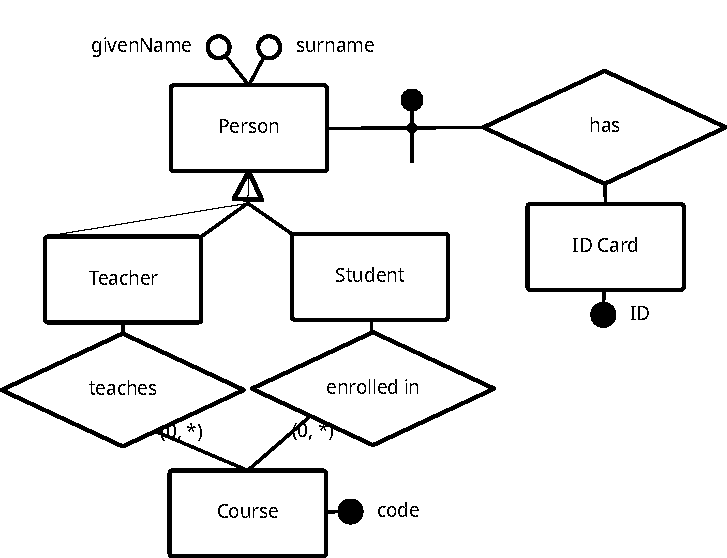
\includegraphics[width=1\textwidth]{./images/university-er.pdf}
            \caption{Entity-Relationship}
            \label{fig:diagrams:er}
          \end{subfigure}
          \begin{subfigure}{0.45\textwidth}
            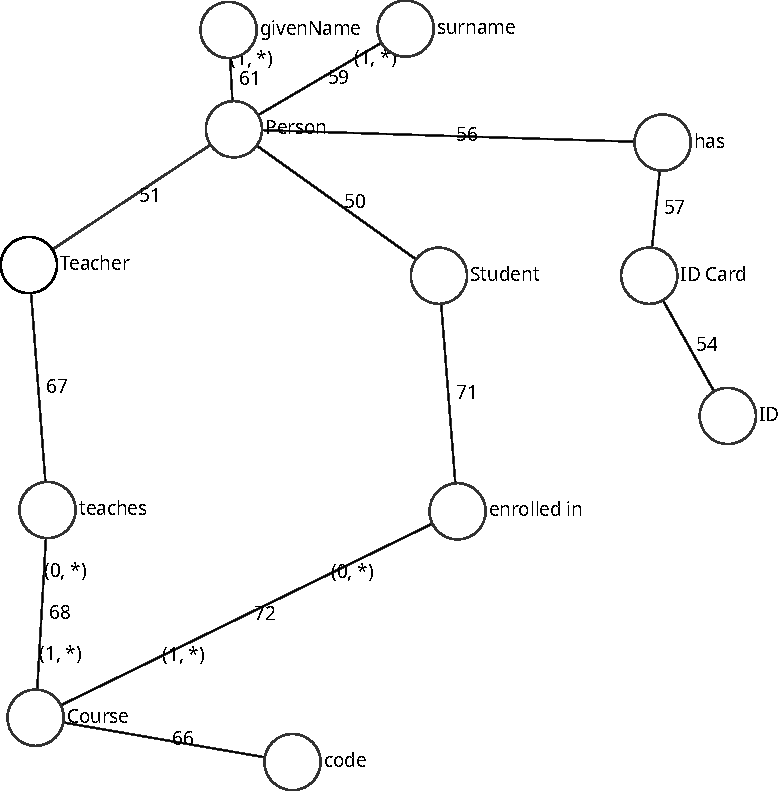
\includegraphics[width=\textwidth]{./images/university-schemcat.pdf}
            \caption{Schematická kategorie}
            \label{fig:diagrams:schemcat}
          \end{subfigure}
          \begin{subfigure}{0.5\textwidth}
            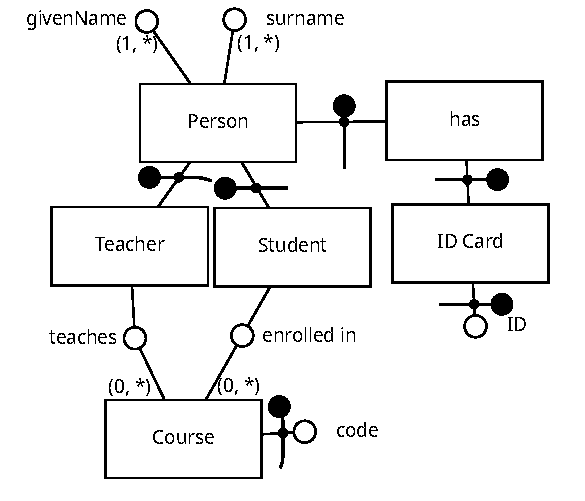
\includegraphics[width=\textwidth]{./images/university-scv.pdf}
            \caption{Vizualizace schematické kategorie}
            \label{fig:diagrams:scv}
          \end{subfigure}
          \caption{Diagramy}
          \label{fig:diagrams}
        \end{figure}

        Na Obrázku~\ref{fig:diagrams:er} je ER schéma vysoké školy s učiteli a studenty, kteří učí resp. docházejí na lekce.
        Odpovídající schematická kategorie je na Obrázku~\ref{fig:diagrams:schemcat}.
        Ta však nevyobrazuje úplně všechna data, která schematická kategorie obsahuje.
        Uživatel je může prozkoumat zvolením jednotlivých objektů nebo morfismů.

        Aby byla jednodušeji z diagramu vidět sémantika schematické kategorie, byla navržena vizualizace schematické kategorie, viz Obrázek~\ref{fig:diagrams:scv}.
      \end{block}
    \end{column}


    \begin{column}{0.5\textwidth - 1.5cm}
      \begin{block}{Uživatelské rozhraní}
        \begin{figure}
          \centering
          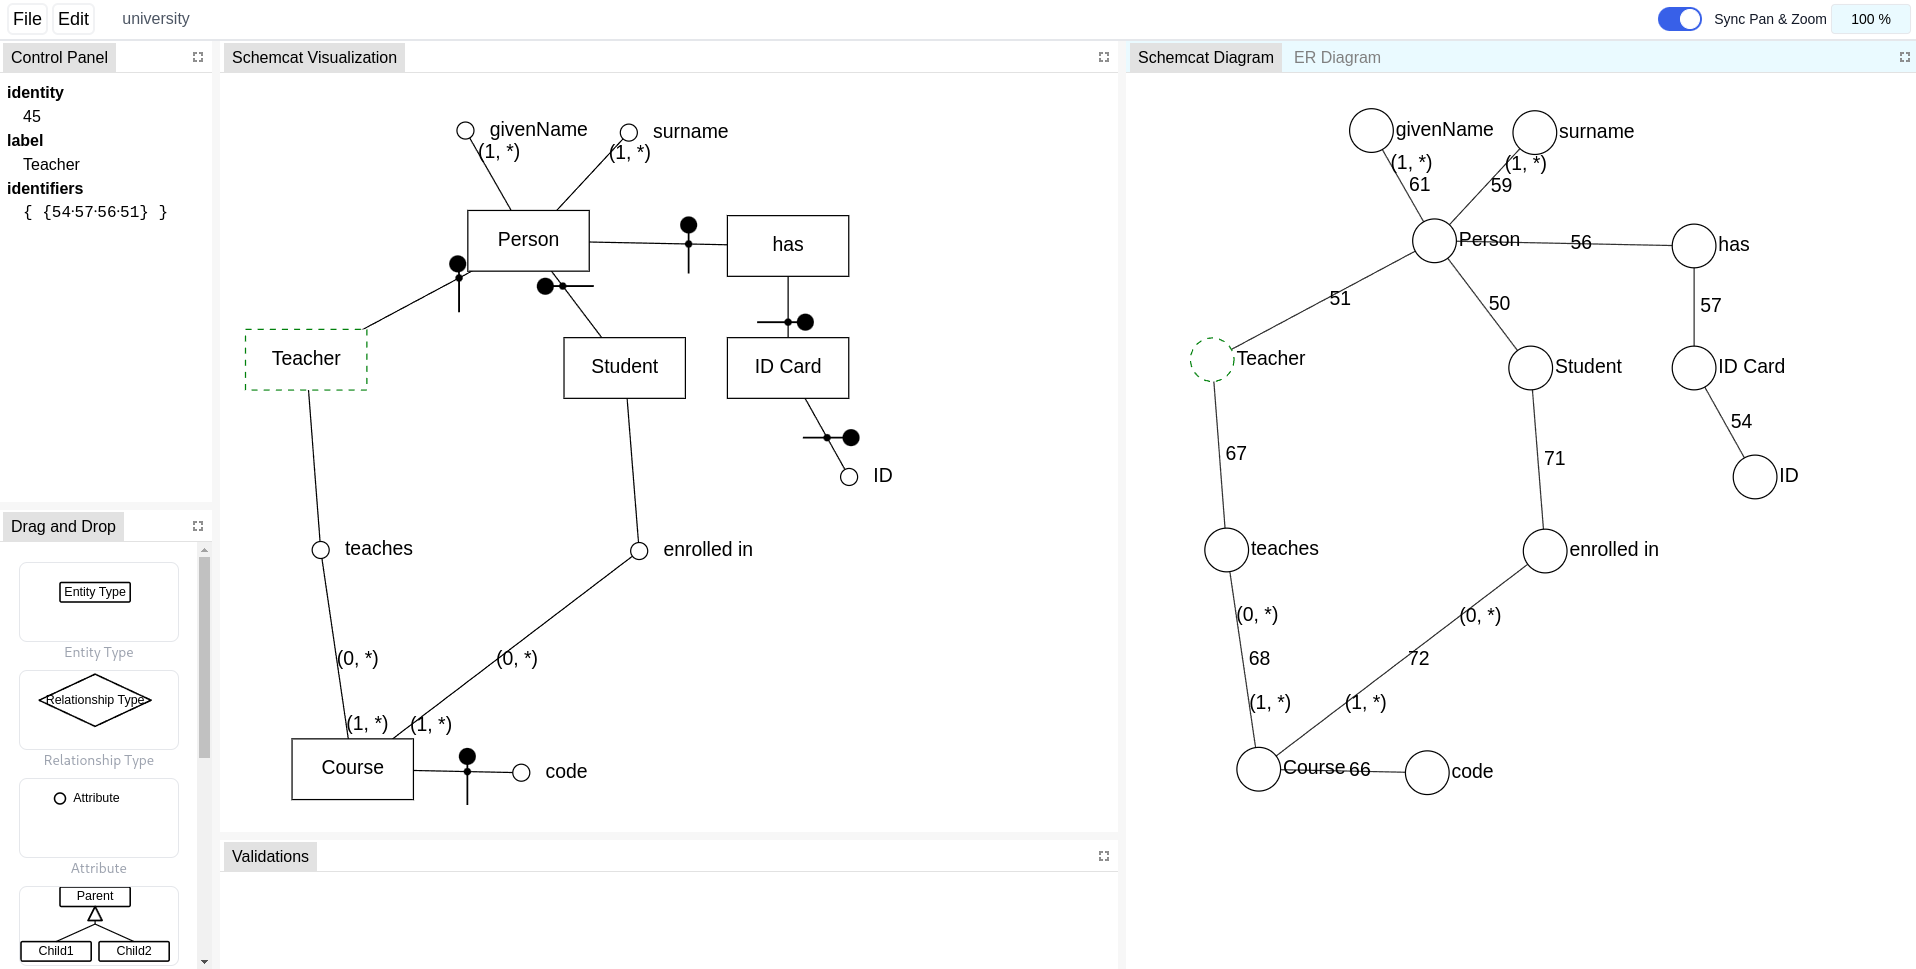
\includegraphics[width=0.8\textwidth]{./images/identifier-screenshot.png}
          \caption{Uživatelské rozhraní}
          \label{fig:user-interface}
        \end{figure}

        Uživatelské rozhraní z Obrázku~\ref{fig:user-interface} je složeno z oken a záložek, které lze libovolně přesouvat a měnit jejich velikost.
        Na obrázku je právě zvolen objekt odpovídající entitě učitele a v ovládacím panelu vlevo lze vidět jeho identifikátor $54\cdot 57\cdot 56\cdot 51$.
        To je řetězec složený ze signatur morfismů, které vedou do objektu, jímž je učitel identifikován (ID identifikační karty).

        Vlevo dole vidíme různé předpřipravené konstrukty, které lze přetažením myší vložit do ER diagramu.

        Dole je (prázdný) seznam validací, který potenciálně ukazuje některé detekované chyby v ER diagramu, které by způsobovaly, že diagram není validní (např.~existující cyklus slabé identifikace).
      \end{block}
      \begin{block}{Závěr}
        Funkcionalita aplikace je dostačující k seznámení s konceptem schematických kategorií.
        Bohužel zvolený framework (React) a knihovny kladly na architekturu a datový model určitá omezení, která jsou v práci definovaná.

        Webová aplikace byla přesto navržena tak, aby umožnila potenciální rozšíření.
        Například:
        \begin{itemize}
          \item UML modelování,
          \item přímá tvorba a úprava schematických kategorií,
          \item online interaktivní spolupráce na tvorbě schémat.
        \end{itemize}
      \end{block}
      \begin{block}{Odkazy}
        \begin{tabular}{rll}
          \qrcode[link,padding,hyperlink,height=3cm]{https://sorashi.github.io/schemcat}  & \href{https://sorashi.github.io/schemcat}{\texttt{sorashi.github.io/schemcat}}   & aplikace     \\
          \qrcode[link,padding,hyperlink,height=3cm]{https://github.com/sorashi/schemcat} & \href{https://github.com/sorashi/schemcat}{\texttt{github.com/sorashi/schemcat}} & zdrojový kód \\
          \qrcode[link,padding,hyperlink,height=3cm]{mailto:prazak.dennis@gmail.com}      & \href{mailto:prazak.dennis@gmail.com}{\texttt{prazak.dennis@gmail.com}}          & email
        \end{tabular}
      \end{block}
    \end{column}
  \end{columns}


  \begin{textblock}{0.5}(0.63, 0.935)
    \color{white}
    \sffamily
    \begin{tabular}{rl}
      Vedoucí:    & RNDr.~Martin Svoboda,~PhD.
      \\
      Pracoviště: & Katedra softwarového inženýrství
    \end{tabular}
  \end{textblock}


\end{frame}
\end{document}
